\subsection{Entity-Relationship Schema}

\begin{center}
    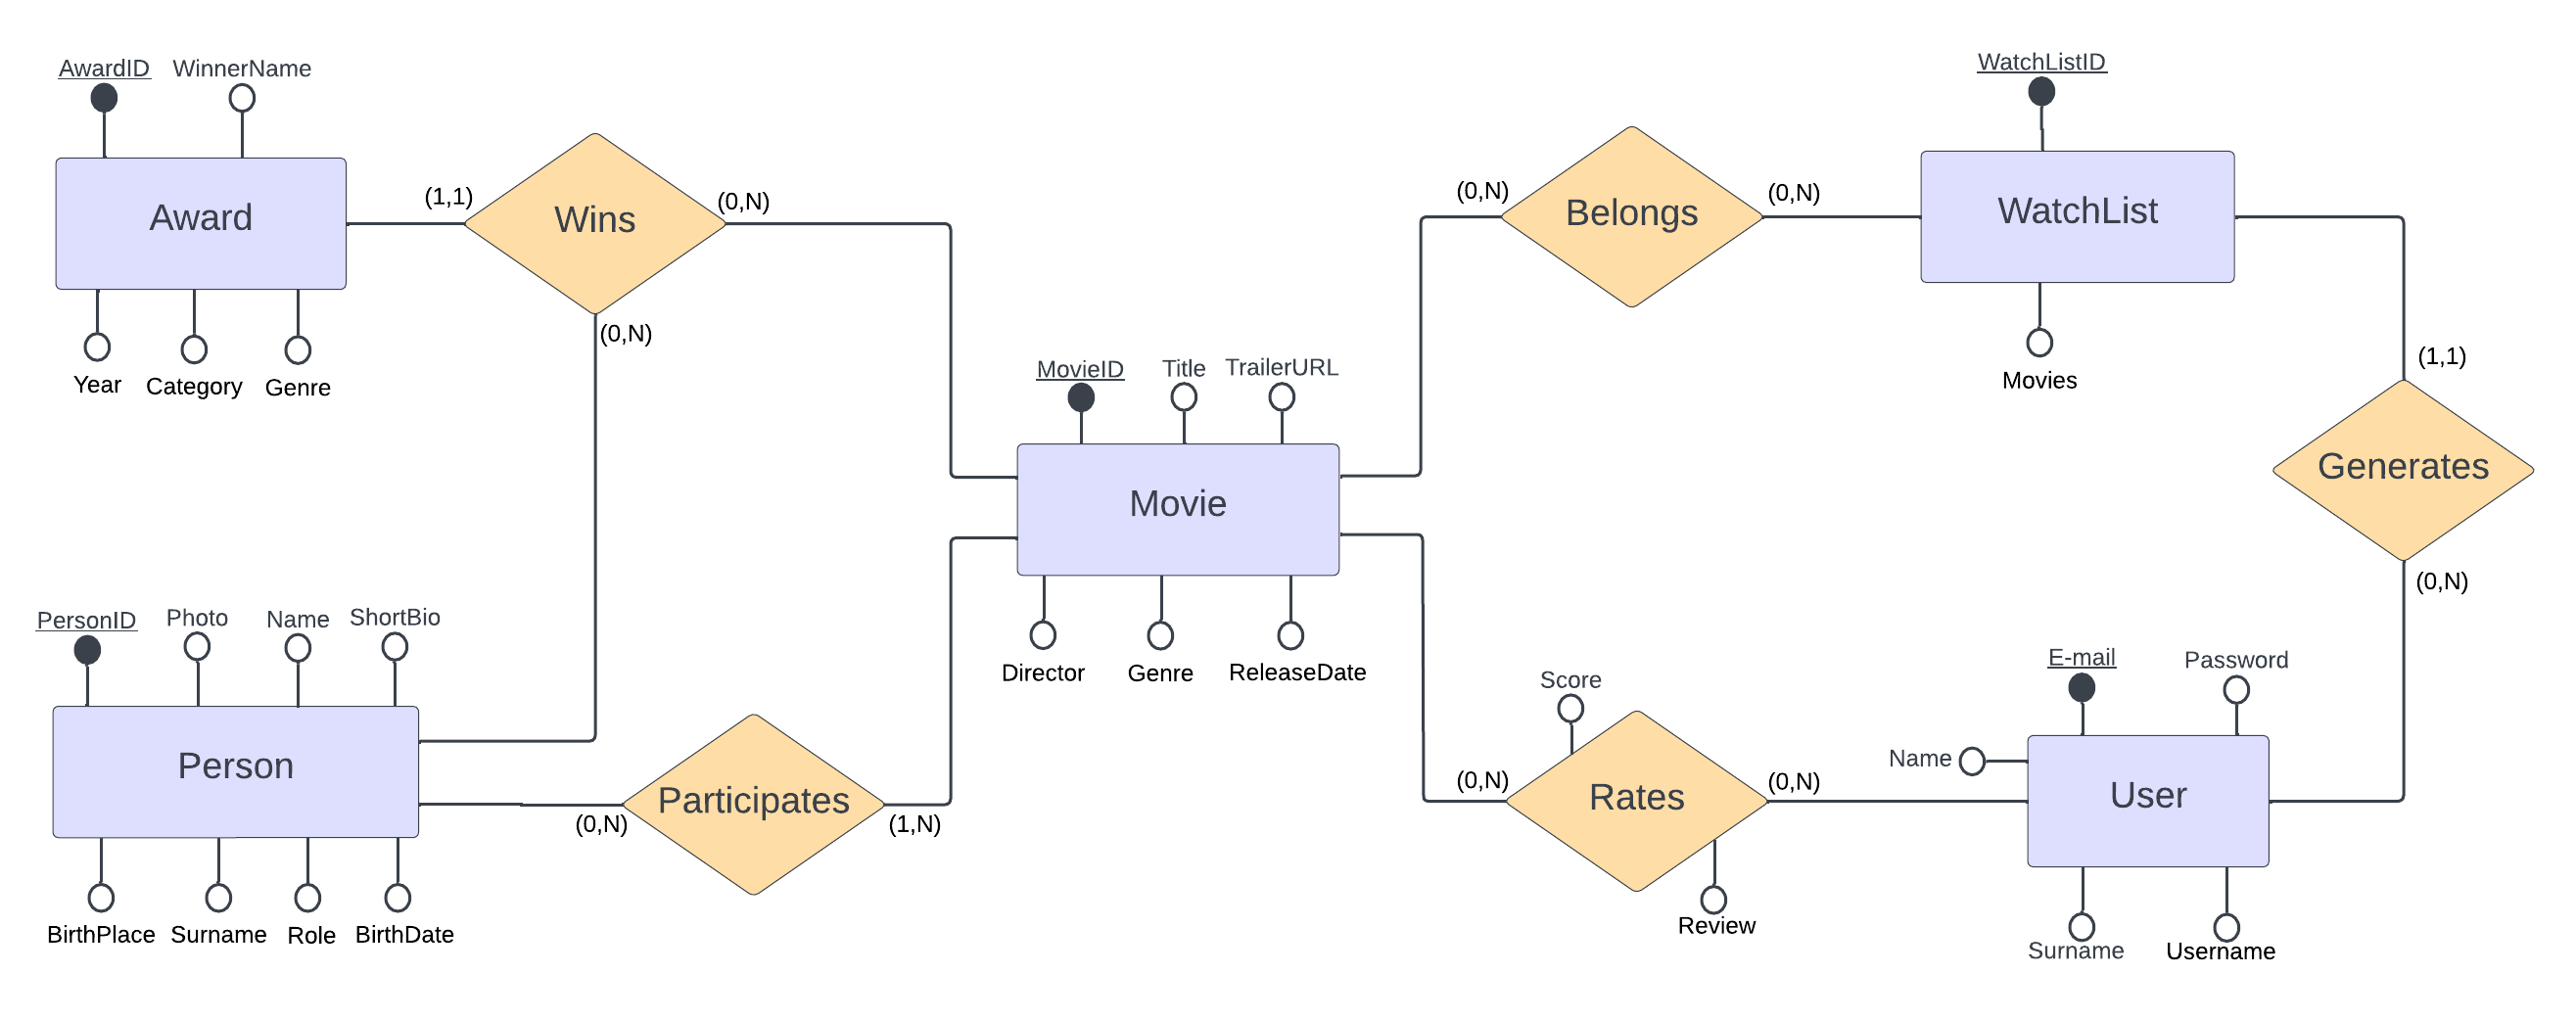
\includegraphics[width=17cm]{pictures/WebEdge-ER-vers07.png}
\end{center}

%Describe here your ER schema

The ER schema contains 5 Entities;
\begin{itemize}

\item \textbf{Movie:} Represents the information about the movies. The primary key is the movie identifier (movieID), which is an INTEGER field. The other attributes are title (TEXT), trailer URL (TEXT), releaseDate (DATE), genre (TEXT), and director (TEXT). All attributes here cannot be null. Each movie should have at least one person, i.e. each movie has a director. So, a movie is participated by 1-N person (with relationship \textit{Participates}). A movie also can win 0-N awards (with relationship \textit{Wins}), belongs to 0-N watchlist (with relationship \textit{Belongs}), and rated by 0-N user (with relationship \textit{Rates}).

\item \textbf{Person:} Represents all actors/actresses/directors/writers/producers that are part of a movie. The primary key is the person identifier (PersonID), which is an INTEGER field. Other attributes include personal information such as name, surname, short biography, birthplace, all having TEXT fields, BirthDate which is a DATE field, and Photo contains a link to the person's photo. The attribute photo can be null, while others cannot. Each person participates 0-N movie (with relationship \textit{Participates}), and can win 0-N awards (with relationship \textit{Wins}).

\item \textbf{User:} Represents all users that are registered on the movie website. The primary key is email, which is a TEXT field. Other attributes include personal information such as name, surname, password, and username, all having TEXT fields. All attributes here cannot be null. Each user can rate 0-N movies (with relationship \textit{Rates}) and generates 0-N watchlists (with relationship \textit{Generates}).

\item \textbf{Award:} Represents all awards that an actress/director has gained. The primary key is Award Identifier (AwardID), which is an INTEGER field. Other attributes are WinnerName, Category, Genre all having TEXT fields, and Year, which is a DATE field. Each award is in a 1-1 relationship with either Movie or Person with turnery relationship \textit{Wins}. As a consequence, Award contains as foreign keys both the movie ID and person ID. If award is won by a movie, then person ID field can be null. If award is won by a person, that person needs to be part of a movie and hence movie ID cannot be null. 

\item \textbf{WatchList:} Represents movies waiting to be watched. The primary key is WatchList Identifier (WatchListID), which is an INTEGER field. Another attribute is movies, which is an array list field. Each watchlist is in a 1-1 relationship with User with binary relationship \textit{Generates}. As a consequence, Watchlist contains as a foreign key of user email and it cannot be null. Each watchlist contains 0-N movies (with relationship \textit{Belongs}). 

\end{itemize}